\title{Introductory Electricity, Magnetism, and Optics Practice Problems}
\author{Cyrus Vandrevala}

\documentclass[11pt]{article}
\usepackage{amsmath}
\usepackage[margin=2.5cm]{geometry}
\usepackage[pdftex]{graphicx}

\begin{document}

\maketitle
\tableofcontents
\vspace{50pt}

\subsection*{Useful Constants}
Electron Mass = $9.11 \times 10^{-31}$ kg \\*
Proton Mass = $1.67 \times 10^{-27}$ kg \\*
Elementary Charge = $1.602 \times 10^{-19}$ C \\*
Coulomb's Constant = $8.99 \times 10^9$ Nm$^2$/C$^2$ \\*
Avogadro's Number = $ 6.02 \times 10^{23}$ atoms/mole \\*\\*

%%%%%%%%%%%%%%%%%%%%%%%%%%%%%%%%%%%%%%%%%%%%%%%%%%%%%%%%%%%%%%%%%%%%%%%%%%%%%%

\pagebreak
\section{Resistors in Circuits}
\vspace{10pt}

\subsection{Resistors in Series}
I place 10 resistors, each with a resistance of $50 \Omega$, in series.  What is the total resistance of the system?\\* \\*
$\Rightarrow 500 \Omega$

\subsection{Resistors in Parallel}
I place 10 resistors, each with a resistance of $50 \Omega$, in parallel.  What is the total resistance of the system?\\* \\*
$\Rightarrow 5 \Omega$

\subsection{Power Through a Resistor}
Two resistors ($10\Omega$ and $20\Omega$) are connected in series to a battery with voltage V = 10 V.  What is power dissipated in the $20\Omega$ resistor?\\* \\*
$\Rightarrow 2.2$ W

\subsection{Maximum Power}
Suppose I have a battery with voltage 100V and an internal resistance of $10\Omega$.  I can hook a resistor of any size in series with this battery.  What is the maximum power that I can possibly deliver to this resistor?\\* \\*
$\Rightarrow$ 250 W

\subsection{Temperature Dependence of a Resistor}
A copper wire has a temperature coefficient $\alpha = 3.93 \times 10^{-3} \Omega/K$ and a resistivity of $1.7 \times 10^{-8} \Omega m$ at 20$^\circ$C.  I extrude a piece of wire that is 1.5 m long with a radius of 1.3 mm.  What is the new resistivity of this wire if I heat it up to 100$^\circ$C?\\* \\*
$\Rightarrow 0.31 \Omega m$

\subsection{Bob's Plight}
Bob the college student is relaxing in his dorm.  Suddenly his mother calls and warns him that she is coming to visit and she will be there in 10 minutes.  Oh no!  His room is a mess!  He must hide his shame!  Without thinking, he leaps up and plugs in his 1000 W vacuum cleaner.  However, he forgot that he already has a 1000 W microwave running with some popcorn, a 600 W coffee maker bubbling away, and a 500 W plasma screen TV playing his favorite show (The Bachelor).  Will he be able to run all of these devices at once?  Or will the 20A fuse blow out, leaving him in the lurch?  You may assume all of these are 120V appliances.\\* \\*
$\Rightarrow$ The fuse will blow, and Bob will be sad...

%%%%%%%%%%%%%%%%%%%%%%%%%%%%%%%%%%%%%%%%%%%%%%%%%%%%%%%%%%%%%%%%%%%%%%%%%%%%%%

\pagebreak
\section{RC Circuits}
\vspace{10pt}

\subsection{Time Constant}
An RC circuit consists of a battery (V = 10V), a resistor (R = 12 $\Omega$), and a capacitor (C = 10 mF) all in series.  What is the time constant of the circuit? \\* \\*
$\Rightarrow$ 0.12 s

\subsection{Charging an RC Circuit}
Suppose I have a simple RC circuit with a time constant of $\tau = 10$ s.  I charge the capacitor to 50\% of its maximum charge.  I then begin to discharge the capacitor.  About how long would it take the capacitor to discharge down to 10\% of its maximum charge?\\* \\*
$\Rightarrow$ 16 s

%%%%%%%%%%%%%%%%%%%%%%%%%%%%%%%%%%%%%%%%%%%%%%%%%%%%%%%%%%%%%%%%%%%%%%%%%%%%%%

\pagebreak
\section{Charges and Currents in Magnetic Fields}
\vspace{10pt}

\subsection{Right Hand Rules \#1}
A positively charged particle travels in the $+\hat{z}$ direction.  There is a magnetic field oriented in the $-\hat{y}$ direction.  In which direction will this particle feel a force? \\* \\*
$\Rightarrow +\hat{x}$ direction

\subsection{Right Hand Rules \#2}
A positively charged particle travels in the $+\hat{y}$ direction.  There is a magnetic field oriented in the $-\hat{x}$ direction.  In which direction will this particle feel a force? \\* \\*
$\Rightarrow +\hat{z}$ direction

\subsection{Right Hand Rules \#3}
A negatively charged particle travels in the $-\hat{z}$ direction.  There is a magnetic field oriented in the $+\hat{y}$ direction.  In which direction will this particle feel a force? \\* \\*
$\Rightarrow -\hat{x}$ direction

\subsection{Right Hand Rules \#4}
A negatively charged particle travels in the $-\hat{x}$ direction.  There is a magnetic field oriented in the $-\hat{y}$ direction.  In which direction will this particle feel a force? \\* \\*
$\Rightarrow -\hat{z}$ direction

\subsection{Right Hand Rules \#5}
A positively charged particle travels in the $-\hat{x}$ direction.  There is a magnetic field oriented in the $-\hat{x}$ direction.  In which direction will this particle feel a force? \\* \\*
$\Rightarrow$ The particle will not feel any magnetic force

\subsection{Particle in a Uniform Magnetic Field}
A particle with charge Q = 1.0 mC travels with a velocity $\vec{v} = 10 \hat{x} - 20 \hat{y}$ m/s.  It enters a region of space with a magnetic field given by $\vec{B} = 1.2 \hat{x} + 2.3 \hat{z}$ T.  What is the resulting force on the particle? \\* \\*
$\Rightarrow F = -46\hat{x} - 23\hat{y} + 24\hat{z}$ N

\pagebreak
\subsection{Velocty Selector}
I cross a magnetic field with strength 1.7 T and an electric field with strength 2.8 N/C in order to create a velocity selector.  I fire a beam of particles, each with mass M = 2.1 kg, into the apparatus.  At what speed would you expect particles to pass through if they experience no deflection? \\* \\*
$\Rightarrow v = 0.61$ m/s

\subsection{Particles in a Magnetic Field}
A magnetic field is oriented into the page, and five particles are fired into it from the bottom.  Which particles are positively charged?  Which particles are negatively charged?  Which particles are neutral?  Of the charged particles, which ones have the largest mass?  Which ones have the smallest mass?

\begin{center}
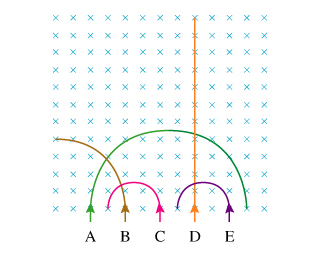
\includegraphics[scale=0.75]{Images/particles_in_magnetic_field.png}
\end{center}

$\Rightarrow$ B, C, and E are positively charged.  A is negatively charged.  D is neutral (no charge).  Since A seems to have the largest arc (just barely bigger than B), it has the largest mass.  Since C and E have the smallest arcs, they are tied for the smallest mass.


%%%%%%%%%%%%%%%%%%%%%%%%%%%%%%%%%%%%%%%%%%%%%%%%%%%%%%%%%%%%%%%%%%%%%%%%%%%%%%

\pagebreak
\section{Biot-Savart Law}
\vspace{10pt}

\subsection{Moving Charged Particle}
A point charge (Q = 1.0 mC) is moving with a velocity $\vec{v} = 3.0 \hat{x}$ m/s.  What is the magnitude of the magnetic field produced by this particle at the point (1 m,1 m) when the particle is located at the origin? \\* \\*
$\Rightarrow B = 1.1 \times 10^{-10}$ T

\subsection{Biot-Savart Law Calculations}
You must know how to find the magnetic field from the following current distributions using the Biot-Savart law.  Please refer to your textbook or class notes for derivations of each of these:

\begin{itemize}
\item Thin Wire Loop
\item Thin Straight Wire
\end{itemize}

%%%%%%%%%%%%%%%%%%%%%%%%%%%%%%%%%%%%%%%%%%%%%%%%%%%%%%%%%%%%%%%%%%%%%%%%%%%%%%

\pagebreak
\section{Ampere's Law}
\vspace{10pt}

\subsection{Four Wires}
Four infinitely long wires have each have a current going into the page or out of the page as shown below.  They are oriented on the corners of a square.  What is the direction of the net magnetic force on wire \#4?

\begin{center}
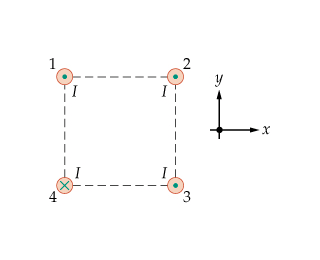
\includegraphics[scale=0.5]{Images/four_wires.png}
\end{center}

$\Rightarrow$ Down and to the Left

\subsection{Ampere's Law Calculations}
You must know how to find the magnetic field from the following current distributions using Ampere's law.  Please refer to your textbook or class notes for derivations of each of these:

\begin{itemize}
\item Infinite Long Thin Wire
\item Infinite Long Thick Wire
\item Infinitely Long Cylindrical Shell
\item Solenoid
\item Toroid
\end{itemize}

%%%%%%%%%%%%%%%%%%%%%%%%%%%%%%%%%%%%%%%%%%%%%%%%%%%%%%%%%%%%%%%%%%%%%%%%%%%%%%

\pagebreak
\section{Magnetic Dipoles}
\vspace{10pt}

\subsection{Loop of Wire in a Magnetic Field}
Suppose I have a wire loop in a uniform magnetic field $\vec{B}$.  The loop has an area A, an area vector $\hat{n}$, and carries a current I.  At what orientation in the field will the loop have a minimum potential energy? \\* \\*
$\Rightarrow$ It will be a minimum when $\hat{n}$ is parallel to $\vec{B}$

\subsection{Vector Analysis}
A magnetic dipole is give by $\vec{\mu} = 10 \hat{z}$ $Am^2$.  It is immersed in a magnetic field given by $\vec{B} = 10 \hat{x} - 50\hat{y}$ T.  What is the magnetic potential energy of the system? \\* \\*
$\Rightarrow$ U = 0 J

%%%%%%%%%%%%%%%%%%%%%%%%%%%%%%%%%%%%%%%%%%%%%%%%%%%%%%%%%%%%%%%%%%%%%%%%%%%%%%

\pagebreak
\section{Vocabulary}
\vspace{10pt}

\subsection{Magnetic Domains}
What type of magnetism is usually associated with magnetic domains? \\* \\*
$\Rightarrow$ Ferromagnetism

\subsection{Conventional Current}
True or False?  Conventional current is the flow of positive charges. \\* \\*
$\Rightarrow$ True

\subsection{Kirichoff's Loop Rule}
True or False?  Kirichoff's loop rule states that the algebraic sum of the voltages around any closed path in a circuit must equal zero. \\* \\*
$\Rightarrow$ True

\subsection{Curie Temperature}
Above the Curie temperature, what type of magnetic materials become paramagnetic? \\* \\*
$\Rightarrow$ Ferromagnetic Materials

%%%%%%%%%%%%%%%%%%%%%%%%%%%%%%%%%%%%%%%%%%%%%%%%%%%%%%%%%%%%%%%%%%%%%%%%%%%%%%

\end{document}




